\documentclass{thesis}

\usepackage{lipsum}

\title{Pico's Thesis}

\author{Valentino Picotti}
\course{Informatica}
\supervisor{Prof.\ Marino Miculan, Ph.D.}
\cosupervisor{Marco Peressotti \and Nicola Gigante}

\begin{document}

\maketitle

\begin{dedication}
Alla mamma <3
\end{dedication}

\begin{abstract}[italian]
%!TEX root = ijcai2016.tex

Facciamo tante belle cose concorrenti
\end{abstract}

\begin{abstract}
%!TEX root = thesis.tex

Transactional memory (TM) has emerged as a promising high-level concurrency control mechanism alternative to fine grained lock-based synchronization.
However, most TM models admit only \emph{isolated} transactions, which are not adequate in multi-threaded programming where transactions have to interact via shared data \emph{before} committing.
In this thesis, we present \emph{Open Transactional Memory} (OTM), a programming model supporting \emph{safe, data-driven} interactions between \emph{composable} memory transactions.
In this model, different transactions are transparently \emph{merged} at runtime as soon as they access to shared variables; their threads can then cooperate, until they all either commit or abort together.
Thus, this model relaxes the isolation requirement still guaranteeing atomicity; moreover, it allows for \emph{loosely-coupled} interactions since transaction merging is dynamic and driven only by accesses to shared data, with no need to specify participants beforehand.

We present OTM in the setting of the Haskell language, taking advantage of its type system for guaranteeing composability.  
After having defined the programmer's interface (i.e., types, data structures and constructs), we give some examples such as barriers and Petri nets; moreover, we show that OTM is a conservative extension of STM.
Finally, we present an implementation of OTM in Haskell, as an alternative of STM.
\end{abstract}

\begin{acknowledgements}[italian]
%!TEX root = thesis.tex

Colgo l’occasione per ringraziare tutte le persone che nel corso di questi tre anni mi hanno dato molto, senza aspettarsi nulla in cambio.

Ringrazio i miei mentori Corral e Giga, da subito rivelatisi ``esempi da seguire'', che con tanta pazienza hanno dato risposta a tutte le mie domande e, giorno dopo giorno, hanno trasformato la mia curiosità per l’Informatica in una vera passione.

Ringrazio Frank per tutti i bei momenti trascorsi assieme durante il primo anno, fatto di poco studio e tanto divertimento: le serate universitarie, la stagione sciistica, gli eventi più disparati e le migliori bevute, avventure e disavventure che hanno fatto maturare una grande amicizia.

Ringrazio Colle, il ``ritrovato'' compagno di studi con cui ho condiviso buona parte del mio percorso universitario, per aver reso produttive, piacevoli ed entusiasmanti le tante ore di studio trascorse insieme e per essere sempre attento alle necessità degli altri.

Ringrazio Corral, Colle e Giga per essere veri amici, sempre presenti con una parola di conforto, una battuta o un consiglio, una stretta di mano o un abbraccio, una serata in compagnia o una nerdata.

Ringrazio, in ordine casuale, i membri dell’Associazione Cultura Informatica: Luca, Federico, Lorenzo, Marta, Alex, Darko e i già citati Corral, Giga e Colle, che rendono l’associazione un piacevole punto di ritrovo per lo studio, gli scambi culturali e i momenti conviviali.

Ringrazio i correlatori Dott. Nicola Gigante e Dott. Marco Peressotti per il contributo dato nella stesura della tesi ed il Prof. Marino Miculan per avermi permesso di lavorare su un progetto molto interessante. 

Infine ringrazio i miei genitori per avermi dato l’opportunità di raggiungere questo traguardo e tutti i familiari per avermi sempre sostenuto ed incoraggiato in questo percorso.
\end{acknowledgements}

\tableofcontents

\mainmatter
%!TEX root = thesis.tex

\chapter{Introduction}

The advent of multi-core architectures has emphasized the crucial importance of mechanisms supporting correct and scalable multi-threaded programming.
In this model, threads can collaborate by interacting on data structures (such as tables, message queues, buffers, etc.) maintained in shared memory.

Traditional lock-based mechanisms (like mutex constructs, semaphores, and barriers) used to regulate access to these shared data are notoriously difficult and error-prone, as they easily lead to deadlocks, race conditions and priority inversions; moreover, they are not composable and hinder parallelism, thus reducing efficiency and scalability.
\emph{Transactional memory} (TM) has emerged as a promising mechanism to replace locks \cite{moss:transactionalmemorybook,st:dc1997}.  The basic idea is to mark blocks of code as \emph{atomic}; then, execution of each block will appear either if it was executed instantaneously at some unique point in time, or, if aborted, as if it did not execute at all. This is obtained by means of \emph{optimistic} executions: the blocks are allowed to run concurrently, and eventually if an interference is detected a transaction is restarted and its effects are rolled back.
Transactions are composable and ensure absence of deadlocks and  priority inversions, automatic roll-back on exceptions, and increased concurrency.  Each transaction can be viewed in isolation as a \emph{single-threaded} computation, significantly reducing programmer's burden.

\section{Motivations}

In multi-threaded programming different transactions may need to interact and exchange data \emph{before} committing.
In this situation, transaction isolation is a severe shortcoming.
A simple example is a request-response interaction via a shared buffer.
We could try to synchronize the threads accessing the buffer \emph{b} by means of two semaphores \verb|c1|, \verb|c2| as follows:
\\[0.6ex]
\begin{BVerbatim}[baseline=t]
// Party1 (Master)
atomically {
  // put request in b
  up(c1);
  // some other code
  down(c2);
  // get answer from b
}
\end{BVerbatim}
\hfill
\begin{BVerbatim}[baseline=t]
// Party2 (Worker)
atomically {
  // some code before
  down(c1);
  // get request from b
  // put answer in b
  up(c2);
  // some code after
}
\end{BVerbatim}
% \\[0.6ex]

Unfortunately, this solution does not work: any admissible execution requires an interleaved scheduling between the two transactions, thus violating isolation; hence, the transactions deadlock as none of them can progress.
It is important to notice that this deadlock arises because synchronization occurs between threads in \emph{different} transactions;
in fact, the solution above is perfectly fine for threads \emph{outside} transactions, or within the \emph{same} transaction.
%As mentioned in \cite{hmpm:ppopp2005}, ``two threads can easily deadlock if each awaits some communication from the other''.


% Paragraph 3: Contribution
\section{Thesis proposal}
In order to overcome this limitation, in this thesis we propose a programming model for \emph{safe, data-driven} interactions between memory transactions.
%whose formal semantic is defined in \citep{OpenTransactionsSpec}.
The key observation is that \emph{atomicity} and \emph{isolation} should be seen as two disjoint computational aspects:
\begin{itemize}
\item an atomic \emph{non-isolated} block of code is executed ``all-or-nothing'', but its execution can overlap that of others and \emph{uncontrolled} access to shared data is allowed;
\item an \emph{isolated} block of code is intended to be executed ``as it were the only one'' (i.e., in mutual exclusion with other threads), but no rollback on errors/exceptions is provided.
\end{itemize}
Thus, a ``normal'' block of code is neither atomic nor isolated; a mutex block (like Java \emph{synchronized} methods) is isolated but not atomic; and a usual transaction is a block which is both atomic and isolated.
%Our claim is that
Atomic non-isolated blocks can be fruitfully used for implementing safe composable interacting memory transactions, henceforth called \emph{open transactions}.

In this model, a transaction is composed by several threads, called \emph{participants}, which can cooperate on shared data.  A transaction commits when all its participants commit, and aborts if any thread aborts.  Threads participating to different transactions can access to shared data, but when this happens the transactions are \emph{transparently merged} into a single one.  For instance, the two transactions of the synchronization example above would automatically merge becoming the same transaction, so that the two threads can synchronize and proceed.  Thus, this model relaxes the isolation requirement still guaranteeing atomicity and consistency; moreover, it allows for \emph{loosely-coupled} interactions since transaction merging is driven only by run-time accesses to shared data, without any explicit coordination among the participants beforehand.

This concepts have already been presented in \cite{MiculanPT15,Toneguzzo,OpenTransactionsSpec}, so in this thesis we not present the operational semantics of the model and the \emph{opacity} correctness criterion\cite{gk:ppopp08}.

In summary, the contributions of this thesis are the following:
\begin{itemize}
\item We present \emph{Open Transactional Memory}, a transactional memory model where multi-threaded transactions can interact by non-isolated access to shared data. Consistency and atomicity are ensured by transparently \emph{merging} transactions at runtime.

\item We describe this model in the context of Concurrent Haskell (\cref{chap:otm}).
We define two monads \emph{OTM} and \emph{ITM}, representing the computational aspects of atomic \emph{multi-threaded open} (i.e., non-isolated) transactions and atomic \emph{single-threaded isolated} transactions, respectively (Figure~\ref{fig:acid-spectrum}).
Using the construct \emph{atomic}, programs in the \emph{OTM} monad are executed ``all-or-nothing'' but without isolation; hence these transactions can merge at runtime.
When needed, isolation inside transactions can be guaranteed by the construct \textcode{isolated}.
Both OTM and ITM transactions are \emph{composable},
and we exploit Haskell type system to forbid irreversible effects inside these two monads.

\item We illustrate the effectiveness of this programming model by providing several example implementations, such as barriers, \emph{futures} and Petri nets, among others.
Moreover, \emph{OTM} is a conservative extension 
of \emph{STM} \citep{Harris:2005:CMT:1065944.1065952}; in fact, \emph{atomically} is precisely the composition of \emph{atomic} and \emph{isolated} (Figure~\ref{fig:acid-spectrum}).

\item We give an implementation of OTM as a library for Concurrent Haskell (\cref{chap:implementation}).  Ours is a pure software implementation using some functionalities of the Haskell Runtime System, and does not require any change in the compiler or the runtime environment. Furthermore, our implementation can be easily integrated in the Runtime System with minimal changes to STM data structures.
\end{itemize}


\begin{figure}
    \centering
    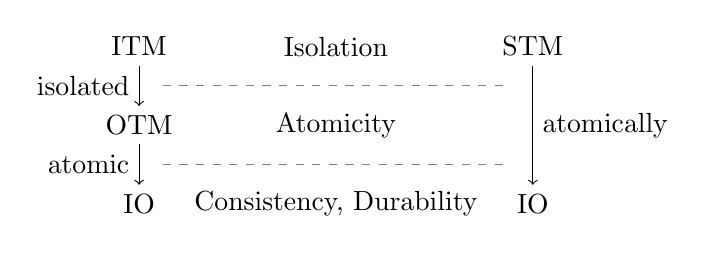
\begin{tikzpicture}
        \node[] (n00) at (0,0) {IO};
        \node[] (n01) at (0,1) {OTM};
        \node[] (n02) at (0,2) {ITM};

        \draw[->] (n02) to node[left] {\textcode{isolated}} (n01);
        \draw[->] (n01) to node[left] {\textcode{atomic}} (n00);

        \node[] (n20) at (5,0)  {IO};
        \node[] (n21) at (5,2){STM};

        \draw[->] (n21) to node[right] {\textcode{atomically}} (n20);

        \node[] (n10) at (2.5,0) {Consistency, Durability};
        \node[] (n11) at (2.5,1) {Atomicity};
        \node[] (n12) at (2.5,2) {Isolation};

        \draw[gray,dashed] (.3,.5) -- (4.7,.5);
        \draw[gray,dashed] (.3,1.5) -- (4.7,1.5);
    \end{tikzpicture}
    \caption{ACID computations: splitting \textcode{atomically}.}
    \label{fig:acid-spectrum}
\end{figure}

\section{Synopsis}
\begin{itemize}
\item In the \cref{chap:haskell} we illustrate the Haskell programming language and the solutions it provides for internal concurrency.

\item In the \cref{chap:otm} we present the programming interface of the OTM model among several example implementations of synchronization primitives and coordination paradigms.

\item In the \cref{chap:ghc} we give an overview of the Haskell compiler, the runtime support and the STM implementation.

\item In the \cref{chap:implementation} we illustrate the implementation of the OTM model.

\item Conclusions and possible future works are illustrated in \cref{chap:conc}.
\end{itemize}

%!TEX root = thesis.tex

\chapter{Haskell and Concurrency}
\label{chap:haskell}

Haskell is a functional programming language, whose syntax and semantics are defined in the ``Haskell Report'' of which the latest revision is Haskell 2010 \cite{Marlow_haskell2010}. Haskell was created by several academic researchers interested in functional languages, to address the lack of a common language that could be used as a focus for their research.

Two features make it stand out amongst the programming languages crowd:
\begin{itemize}
\item It is \emph{purely functional}, \ie functions can not have side effects or mutate data; for a given input a function always gives the same result.
\item It is \emph{lazy}. Unlike the majority of the programming languages, Haskell does not use strict evaluation, in which the arguments of a function are evaluated before the function is called. In Haskell the arguments to a function are passed \emph{unevaluated}, and only evaluated on demand.
\end{itemize}

I/O operations do not fit the functional paradigm because side effects are not permitted and laziness gives deliberately unspecified order of evaluation.

In Haskell, reconciling I/O operations with this features has been achieved by means the IO monad \cite{PeytonJones:1993:IFP:158511.158524}.
\begin{figure}
\begin{lstlisting}
newtype IO a = IO (State# RealWorld -> (# State# RealWorld, a #))
\end{lstlisting}
\caption{IO type definition}
\label{fig:io}
\end{figure}
As shown in \cref{fig:io}, a value of type \emph{IO a} is a monadic action implemented as a function which takes as its input a value representing the entire current state of the world and returns a pair consisting of a value representing the new state of the world, and the result of type \emph{a}.
This introduces \emph{data dependency} between monadic actions, because each action depends on the \emph{RealWord} value computed by the previous one, hence, preventing the compiler from reordering actions, \emph{sequencing} is introduced for I/O operations.
Besides I/O operations, values of IO include operations with side effects on mutable data types, \eg, a mutable variable has type \emph{IORef a} and may be accessed only via the following operations:

\begin{lstlisting}
newIORef   :: a -> IO (IORef a)
readIORef  :: IORef a -> IO a
writeIORef :: IORef a -> a -> IO ()
\end{lstlisting}

\section{Concurrent Haskell}
Concurrent Haskell is the collective name for the facilities that Haskell provides for programming with \emph{internal concurrency}.
It extends the Haskell Language Report adding explicit concurrency primitives to the IO Monad.
Haskell threads are created by \emph{forkIO} that takes as argument the IO computation to be performed independently from the main execution path.
\begin{lstlisting}
forkIO   :: IO () -> IO ThreadId
\end{lstlisting}

Thread safe communication and synchronization is achieved through \emph{MVars}.
A value of type \emph{MVar a} is a mutable location that is either empty or full with a value of type \emph{a}.
Interaction with \emph{MVars} is possible only with the primitives:
\begin{lstlisting}
takeMVar :: MVar a -> IO a
putMVar  :: MVar a -> a -> IO ()
\end{lstlisting}
The first empties a full \emph{MVar}, if it is empty the thread waits until is filled. The second fills an empty \emph{MVar} and blocks the thread if it is full. \emph{MVars} can be though as one place channels, or as binary semaphores for thread synchronization.

\section{Haskell STM}
\label{sec:stm}
Haskell STM is part of Concurrent Haskell, and adds \emph{transactional actions} that operate on \emph{transactional memory} for safe thread communication. Transactional memory locations are called \emph{transactional variables} or \emph{TVars}.
Transactional actions have type \emph{STM a} and are combined sequentially with the bind operator.
An STM action is provisional during its entire execution and its effects are exposed to the rest of the system by 
\begin{lstlisting}
atomically :: STM a -> IO a
\end{lstlisting}
which takes an STM action and delivers an I/O action that, when performed, runs the transaction guaranteeing atomicity and isolation with respect to the rest of the system.
The type system ensure that IO actions can not be performed inside a transaction, so no irreversible side effects can occur inside the STM monad.

\emph{Transactional variables} have type \emph{TVar a}, where \emph{a} is the type of the value they contain. \emph{TVars} are mutable variables so, like IORefs, they are manipulated only via the interface:
\begin{lstlisting}
newTVar   :: a -> STM (TVar a)
readTVar  :: TVar a -> STM a
writeTVar :: TVar a -> a -> STM ()
\end{lstlisting}

Reads and writes on transactional variables can be combined with the monadic bind operator to define a transactional update:

\begin{lstlisting}
modifyTVar :: TVar a -> (a -> a) -> STM ()
modifyTVar var f = do
    x <- readTVar var
    writeTVar var (f x)
\end{lstlisting}

Then, \emph{atomically (modifyTVar x f)} delivers an IO action that applies \emph{f} to the value held by \emph{x} and updates the variable accordingly as a single atomic isolated operation.

Besides transactional memory interaction, STM allows also for \emph{composable blocking} of transactions with the primitive:

\begin{lstlisting}
retry :: STM a
\end{lstlisting}

The composability property, comes from its type that allows the primitive to be used wherever an STM action may occur.
The semantic of \emph{retry} is to abort the transaction and re-run it after at least one of the transactional variables it has read from has been updated.
As shown in \cite{Harris:2005:CMT:1065944.1065952}, this blocking primitive is enough to implement \emph{MVars} using STM: a value of type \emph{MVar a} is a transactional variable holding a value of type \emph{Maybe a}, i.e. a type that is either \emph{Nothing} or actually holds something of type \emph{a}. A thread applying \emph{takeMVar} to an empty \emph{MVar} is effectively blocked since it retries the transaction upon reading \emph{Nothing} and then it is not rescheduled until the content of the transactional variable changes:

\begin{lstlisting}
type MVar a = TVar (Maybe a)
takeMVar v = do
    m <- readTVar v
    case m of
        Nothing -> retry
        Just r -> writeTVar m Nothing >> return r
\end{lstlisting}

Besides the bind operator, that sequentially combines transactions, the primitive:
\begin{lstlisting}
orElse :: STM a -> STM a -> STM a
\end{lstlisting}
combines transactions as \emph{alternatives}. The \emph{orElse} executes the first transaction, if it retries then is abandoned with no effect and the second is started. If the second retries too, the entire call retries and waits on the variables read by either of the two nested transactions.  

%!TEX root = thesis.tex

\chapter{Open Memory Transactions in Haskell}
\label{chap:otm}
In this chapter we present the OTM model and his interface in Haskell.
Haskell was chosen as the development language because of its very expressive type system that offers a perfect environment for studying the ideas of transactional memory.
In \cite{Harris:2005:CMT:1065944.1065952} this has been used to single out computations which may be used in transactions, from those which can perform irreversible I/O effects. 
In the implementation, this idea is further improved by using the type system to separate \emph{isolated} transactions from those who can interact, and hence be merged.

\begin{figure}
    \centering
    \begin{Verbatim}[tabsize=3, gobble=2]
        data ITM a
        data OTM a
        -- henceforth, t is a placeholder for ITM or OTM --
        
        -- Sequencing, do notation ------------------------
        (>>=)  :: t a -> (a -> t b) -> t b
        return :: a -> t a
        
        -- Running isolated and atomic computations -------
        atomic   :: OTM a -> IO a
        isolated :: ITM a -> OTM a
        
        -- Composing transactions -------------------------
        class (Monad m) => MonadTransaction m where
            retry    :: m a
            orElse   :: m a -> m a -> m a
        
        -- Exceptions -------------------------------------
        throw :: Exception e => e -> t a
        catch :: Exception e => t a -> (e -> t a) -> t a
        
        -- Threading --------------------------------------
        fork :: OTM () -> OTM ThreadId
        
        -- Transactional memory ---------------------------
        data OTVar a
        class (Monad m) => MonadTM m where
            newOTVar     :: a -> m (OTVar a)
            readOTVar    :: OTVar a -> m a
            writeOTVar   :: OTVar a -> a -> m ()

    \end{Verbatim}
    \caption{The base interface of OTM.}
    \label{fig:base-interface}
\end{figure}

\section{Transactional actions and variables}
The key idea introduced by \citet{OpenTransactionsSpec} is to separate isolation from atomicity: isolation is a computational aspect that can be added to atomic transactions.
Following this perspective, at the type system level we distinguish isolated atomic actions, represented as values of type \emph{ITM a}, and non isolated atomic actions, as values of type \emph{OTM a}. Actions can be sequentially composed with the corresponding bind operator preserving atomicity and, for ITM actions, isolation.

The function \textcode{isolated} takes an isolated atomic action and delivers an atomic action whose effects are guaranteed to be executed in isolation with respect to other actions.
Then, \emph{atomic} takes an atomic action and delivers an I/O action that when performed runs a transaction whose effects are kept tentative until it commits.
Tentative effects are shared among all non isolated transactions. Values of type \emph{STM a} can be seen as values of type \emph{ITM a}: the I/O they deliver is the same, since \emph{atomically} can be expressed as:
\begin{lstlisting}
    atomically = atomic . isolated
\end{lstlisting}

Like \emph{STM}, \emph{OTM} provides a mechanism for safe thread
communication by means of transactional variables called \emph{OTVars}
which, differently from TVars, support \emph{open} transactions.
These are values of type \emph{OTVar a} where \emph{a} is the type of value held.
Creating, reading and writing \emph{OTVars} is done via the interface defined by the \emph{MonadTM} class shown in \cref{fig:base-interface}. 
All these actions are both atomic and isolated, thus, when it comes to actions of type \emph{ITM a}, \emph{OTVars} are basically \emph{TVars};
\eg \emph{modifyTVar} from \emph{STM} corresponds to:
\begin{lstlisting}
    modifyOTVar :: OTVar a -> (a -> a) -> ITM ()
    modifyOTVar var f = do
        x <- readOTVar var
        writeOTVar var (f x) 
\end{lstlisting}
From its type it is immediate to see that the update is both atomic and isolated. In fact, read and write operations are glued together by the \textgreater \textgreater= combinator, preserving both properties.

\section{Blocking}
\emph{OTM} supports composable blocking via the primitive \textcode{retry}, 
under \emph{STM} slogan ``a thread that has to be blocked because it has 
been scheduled too soon''. As for \emph{STM}, retrying a transactional action 
actually corresponds to block the threads on some condition. Both isolated and non-isolated transactions are instances of \emph{MonadTransaction} class described in \cref{fig:base-interface}.

Checks may be declared as follows:
\begin{lstlisting}
check :: Bool -> ITM ()
check b = if b then return () else retry
\end{lstlisting}
and invariants on transactional variables can be easily checked by composing reads and checks as follow:
\begin{lstlisting}
assertOTVar :: OTVar a -> (a -> Bool) -> ITM ()
assertOTVar var p = do
    x <- readOTVar var
    check (p x)
\end{lstlisting}

Synchronization primitives, such as semaphores, can be easily implemented with isolated actions.
A semaphore is a counter with two fundamental operations: \emph{up} which increments the counter and \emph{down} which decrements the counter if it is not zero and blocks otherwise.
Semaphores are implemented using \emph{OTM} as \emph{OTVars} holding a counter:
\begin{lstlisting}
type Semaphore = OTVar Int
\end{lstlisting}
Then, \textcode{up} and \textcode{down} are even more immediate than their description:
\begin{lstlisting}
up :: Semaphore -> ITM ()
up var = modifyOTvar var (1+)

down :: Semaphore -> ITM ()
down var = do
    assertOTVar var (> 0)
    modifyOTVar var (-1+)
\end{lstlisting}
Both are atomic and isolated updates with the latter being guarded by a pre-condition.

Actions can also be composed as \emph{alternatives} by means of the primitive \emph{orElse}. For instance, the following takes a family of semaphores and delivers an action that decrements one of them, and blocking only if none can be decremented:
\begin{lstlisting}[language=haskell]
downAny :: [Semaphore] -> ITM ()
downAny (x:xs) = down x `orElse` downAny xs
downAny [] = retry
\end{lstlisting}

\section{Thread interaction}

The interchangeability of \emph{OTM} and \emph{STM} ends when isolation is dropped.
\emph{OTM} offers shared \emph{OTVars} as a mechanism for safe \emph{transaction interaction}.
This means that non-isolated transactional actions see the effects on shared variables of any other non-isolated transactional action, as they are performed concurrently on the same object.
This introduces dependencies between concurrent tentative actions: an action can not make its effects permanent, if it depends on information produced by another action which fails to complete.
\emph{OTM} guarantees coherence of transactional actions in presence of interaction through shared transactional variables.

%Among several ways for threads to communicate and coordinate, OTVars enables loosely-coupled interaction right inside atomic actions taking the programming style of \emph{STM} a step further. 
A synchronization scenario that highlights how \emph{OTM} can take the programming style of \emph{STM} a step further is described below.

In this example a master process tries to outsource part of an atomic computation to some thread chosen from a worker pool; communication is coordinated by a pair of semaphores.
This can be achieved straightforwardly using \emph{OTM}:\\


\begin{minipage}{0.45\textwidth}
\begin{Verbatim}
        master c1 c2 = do
            -- put request
            isolated (up c1)
            -- do something else
            isolated (down c2)
            -- get answer
\end{Verbatim}
\end{minipage}
\begin{minipage}{0.45\textwidth}
\begin{Verbatim}
        worker c1 c2 = do
            -- do something
            isolated (down c1)
            -- get request
            -- put answer
            isolated (up c2)
\end{Verbatim}
\end{minipage}
\\

Both functions deliver atomic actions that synchronize using
\textcode{c1} and \textcode{c2}. 

\section{Concurrency}

Differently from \emph{STM}, \emph{OTM} supports parallelism inside non-isolated transactions.
We can easily fork new threads without leaving \emph{OTM} but, like any effect of a transactional action, thread creation and execution remain tentative until the whole transaction commits. 
Forked threads participate to their transaction and impact its life-cycle (e.g.~issuing aborts) as any other participant.
This means that before committing, all forked threads have to complete their transactional action, i.e.~terminate.
Therefore, although the whole effect delivered by the transaction has happened concurrently, forked threads  never leave a transaction alive.

% Because of their transactional nature, threads forked inside
% a transaction do not have compensations nor continuations 
% (i.e.~I/O actions to be executed after an abort or after a commit).
% Compensations are pointless since aborts revert all effects including 
% thread creation. It is indeed possible to replace the primitive 
% \textcode{fork} with one supporting I/O actions as continuations like
% \begin{Verbatim}[tabsize=3, xleftmargin=1ex, gobble=1]
%     forkCont :: OTM a -> (a -> IO ()) -> OTM ThreadID
% \end{Verbatim}
% In fact, this mechanism can be implemented with the primitives
% already offered \emph{OTM}:  since commits are synchronisation points,
% the above corresponds to the parent thread
% forking a thread for each continuation, after the atomic action is
% successfully completed.

On the other hand, by definition isolated atomic actions have to appear 
as being executed in a single-threaded setting; hence neither 
\emph{STM} nor \emph{ITM} actions support thread creation.



\section{Examples}
\paragraph{Crowdfunding}
In this example we consider a scenario in which
one party needs to atomically acquire a given number 
of resources which are offered by a dynamic group.
For the sake of exposition we rephrase the example
using the metaphor of a fundraiser's ``crowdfunding campaign'': 
the resources to be acquired are the campaign goal
and the resources are donated by a crowd of \emph{backers}.

\begin{figure}
    \centering
    \begin{Verbatim}[tabsize=3, gobble=2]
        type Account = OTVar Int
        type Campaign = (Account, Int)

        transfer :: Account -> Account -> Int -> ITM ()
        transfer a1 a2 n = do
            withdraw a1 n
            deposit a2 n

        newCampaign target = do
            a <- newOTvar 0
            return (a, target)
        
        backCampaign :: Account -> Campaign -> Int -> ITM ()
        backCampaign a (a',_) k = transfer a a' k
        
        commitCampaign :: Account -> Campaign -> ITM ()
        commitCampaign a (a', t) = do
            x <- readOTVar a'
            check (x >= t)
            transfer a' a x
    \end{Verbatim}
    \caption{Crowdfunding.}
    \label{fig:example-funding}
\end{figure}

Each participant has a bank account, i.e.~an OTVar holding an integer 
representing its balance. Accounts have two operation \textcode{deposit} 
and \textcode{withdraw} which are implemented on the lines of 
\textcode{up} and \textcode{down}, respectively.
A campaign have a temporary account to store funds
before transferring them to the fundraiser that closes
the campaign; this operation blocks until the goal 
is met. % (for simplicity we omitted time constraints).
Backer participants transfer a chosen amount of funds from their
account to the campaign account, but the transfer is delayed until the campaign is closed. Notice that participants do not need to know each other to coordinate.
The implementation is shown in Figure~\ref{fig:example-funding}.

\paragraph{Thread barriers}
Barriers are abstractions used to coordinate groups of threads;
once reached a barrier, threads cannot cross it
until all other participants reach the barrier. 
Thread groups can be either dynamic or static, depending
on whether threads may join % (and in some implementations leave)
the group or not. Here we consider dynamic groups. 

Threads interact with barriers through two base operations: \textcode{join} for  
joining the group associated with the barrier and \textcode{await} for blocking 
waiting all participants before crossing.

\begin{figure}
    \centering
    \begin{Verbatim}[tabsize=3, gobble=2]
        type Barrier = OTVar (Int, Int)

        newBarrier :: ITM Barrier
        newBarrier = newOTVar (0,0)    
    
        join :: Barrier -> ITM ()
        join b = do
            assertOTVar b nobodyWaiting
            modifyOTVar b (bimap (1+) id)
            
        await :: Barrier -> OTM ()
        await b = do
            isolated $ modifyOTVar b (bimap (-1+) (1+))
            isolated $ do
                assertOTVar b nobodyRunning
                modifyOTVar b (bimap id (-1+))
        
        nobodyRunning (r,_) = r == 0
        nobodyWaiting (_,w) = w == 0
        bimap f g (a, b) = (f a, g b)
    \end{Verbatim}
%    \begin{Verbatim}[tabsize=3, gobble=2]
%        type Barrier = OTVar (Int, Int)
%
%        newBarrier :: ITM Barrier
%        newBarrier = newOTVar (0,0)    
%    
%        join :: Barrier -> ITM ()
%        join b = do
%            assertOTVar b nobodyWaiting
%            modifyOTVar b recordJoin
%            
%        await :: Barrier -> OTM ()
%        await b = do
%            isolated $ modifyOTVar b recordAwait
%            isolated $ do
%                assertOTVar b nobodyRunning
%                modifyOTVar b recordLeave
%        
%        nobodyRunning (r,_) = r == 0
%        nobodyWaiting (_,w) = w == 0
%        recordJoin  (r,w) = (r+1,w)
%        recordAwait (r,w) = (r-1,w+1)
%        recordLeave (r,w) = (r,w-1)
%    \end{Verbatim}
%    \begin{Verbatim}[tabsize=3, gobble=2]
%        type Barrier = (OTVar Int, OTVar Int)
%
%        newBarrier :: ITM Barrier
%        newBarrier = do
%            running <- newOTVar 0
%            waiting <- newOTVar 0
%            return (running,waiting)
%            
%        join :: Barrier -> ITM ()
%        join (running,waiting) = do
%            assertOTVar waiting (== 0)
%            modifyOTVar running (1 +)
%            
%        await :: Barrier -> OTM ()
%        await b = do
%            isolated $ do
%                modifyOTVar running (-1 +)
%                modifyOTVar waiting (1 +)
%            isolated $ do
%                assertOTVar running (== 0)
%                modifyOTVar waiting (-1 +)
%    \end{Verbatim}
    \caption{Thread barrier.}
    \label{fig:example-barrier}
\end{figure}

Barriers can be implemented using \emph{OTM} in few lines as shown
in Figure~\ref{fig:example-barrier}. A barrier is composed by
a transactional variable holding a pair of counters 
tracking the number of participating threads that are waiting
or running. For the sake of simplicity, we prevent new joins 
during barrier crossing.
This is enforced by the assertion guarding the counter update
performed by \textcode{join}. 
Waiting and crossing correspond to the two isolated actions composing
\textcode{await}: the first changes the state of the thread from
running to waiting and the second ensures that all threads reached the barrier
before crossing and decrementing the waiting counter.
Differently from \textcode{join}, \textcode{await} cannot
be isolated: isolation would prevent other
participants from updating their state from ``running'' to ``waiting''.

This implementation is meant as a way to coordinate
concurrent transactional actions but it may be used
for coordinating concurrent I/O actions as it is.
The latter scenario could be implemented also using
\emph{STM} although \textcode{await} would necessarily
be an I/O action since it cannot be an
isolated atomic action (i.e., of type \emph{STM\;a}).

\paragraph{Atomic futures}
Suppose we want to delegate some task to another thread and 
then collect the result once it is ready. An intuitive way to 
achieve this is by means of \emph{futures}, i.e.~``proxy results'' 
that will be produced by the worker threads. 

\begin{figure}
    \centering
    \begin{Verbatim}[tabsize=3, gobble=2]
        type Future a = OTVar (Maybe a)
        
        spawn :: OTM a -> OTM (Future a)
        spawn job = do 
            future <- newOTVar Nothing
            fork (worker future)
            return future
            where
                worker :: Future a -> OTM ()
                worker future = do 
                    result <- job
                    writeOTVar future (Just $! result)
                    
        getFuture :: Future a -> ITM a
        getFuture f = 
            v <- readOTVar f
            case v of
                Nothing -> retry
                Just val -> return val        
    \end{Verbatim}
    \caption{Atomic futures.}%$
    \vspace{-1ex}
    \label{fig:example-futures}
\end{figure}

A future can be implemented in \emph{OTM} by a OTVar
holding a value of type \emph{Maybe a}: either it is
``not-ready-yet'' (\textcode{Nothing}) or it holds something 
of type \emph{a}.
Future values are retrieved via \textcode{getFuture} which takes 
a future and delivers an action that blocks until the value is
ready and then produces the value.
Futures are created by \textcode{spawn} which takes a transactional
action to be performed by a forked (transactional) thread. 
The full specification is in Figure~\ref{fig:example-futures}.

\paragraph{Petri nets}
Petri nets are a well-known (graphical) formal model for concurrent, discrete-event dynamic systems.
A Petri net is readily implemented in \emph{OTM} 
by representing each transition by a thread, and each place by a semaphore.
Each thread repeatedly simulates the firing of the transition it 
implements and updates its input and output places accordingly:
putting and taking a token from a place correspond to 
increasing (\textcode{up}) or decreasing (\textcode{down})
its semaphore---the latter blocks if no tokens are available.
These semaphore operations must be 
performed atomically but not in isolation; in fact, 
isolation would prevent transitions sharing a place to
fire concurrently. 
Using \emph{OTM}, all this is achieved in few lines as shown in \cref{fig:petrinets}.\newpage

\begin{figure}
\begin{Verbatim}[tabsize=3, xleftmargin=1ex, gobble=1]
    type Place = Semaphore
    
    transition :: [Place] -> [Place] -> IO ThreadId
    transition inputs outputs = forkIO (forever fire)
        where 
            fire = atomic $ do
                mapM_ (isolated . down) inputs
                mapM_ (isolated . up)   outputs
\end{Verbatim}
\caption{Petri nets}
\label{fig:petrinets}
\end{figure}

Note that, since firing is atomic but not isolated,
the above is an implementation of \emph{true concurrent} Petri nets, which is usually more difficult to achieve than interleaving semantics.

For instance, consider the Petri net below:
\\\\
\noindent
\begin{BVerbatim}[tabsize=3, xleftmargin=1ex, gobble=2]
        main = do
            p1 <- atomic (newPlace 1)
            p2 <- atomic (newPlace 0)
            p3 <- atomic (newPlace 0)
            p4 <- atomic (newPlace 0)
            transition [p1] [p3, p4]
            transition [p1, p2] [p4]
\end{BVerbatim}
\hfill
\begin{minipage}[t]{.33\linewidth}
    \begin{tikzpicture}
        \node [place,tokens=1, label=left:$p_1$] (p1) at (0,2) {};
        \node [place, label=right:$p_2$] (p2) at (1,2) {};
        
        \node [place, label=left:$p_3$] (p3) at (0,0) {};
        \node [place, label=right:$p_4$] (p4) at (1,0) {};
        
        \node [transition,label=left:$t_1$] (t1) at (0,1) {}
            edge [pre]  (p1)
            edge [post] (p3)
            edge [post] (p4);
        
        \node [transition,label=right:$t_2$] (t2) at (1,1) {}
            edge [pre]  (p1)
            edge [pre]  (p2)
            edge [post] (p4);
    \end{tikzpicture}
\end{minipage}
\\[1ex]
Since $p_1$ has only one token either $t_1$ or $t_2$ fires. In fact,
whenever $t_2$ acquires the token it will fail to acquire the other
from $p_2$ and hence its transaction retries releasing the token.
\newpage
\paragraph{Dinning philosophers}
\begin{figure}
    \centering
    \begin{tikzpicture}[rotate=90]
        \def \k {7}
        \def \radius {2cm}
        
        \foreach \s in {1,...,\k} {
            \draw 
                let 
                    \n1={-360/\k * (\s-1)}
                in 
                node [place,tokens=1,rotate=\n1,label=90:$p_\s$] 
                    (p\s) at (\n1:\radius) {};
        }
        \foreach \s in {1,...,\k} {
            \draw 
                let 
                    \n1={int(mod(\s,\k)+1)},
                    \n2={-360/\k * (\s-1) - 360/(\k*2)}
                in 
                node [transition, rotate=\n2,label=90:$t_\s$]
                    (t\s) at 
%                    (\n2:\radius)
                    ($(p\s)!.5!(p\n1)$) 
                    {}
                    edge [pre, bend right]  (p\s)
                    edge [pre, bend left]  (p\n1)
                    edge [post, bend left] (p\s)
                    edge [post, bend right] (p\n1);
        }
    \end{tikzpicture}
    \begin{Verbatim}[tabsize=3, gobble=2]
        philosophers k = pairs >>= mapM_ philosopher
            where
                philosopher (l,r) = transaction [l,r] [l,r] 
                right = atomic . sequence . take k . repeat $ newPlace 1
                left  = take k . drop 1 . cycle <$> right
                pairs = zip <$> right <*> left
    \end{Verbatim}
\caption{Petri's dining philosophers.}
\label{fig:example-petri-philosophers}
\end{figure}

Dijkstra's \emph{dining philosophers problem} is a textbook
classic of concurrency theory. This problem can be modelled using Petri 
nets representing each fork and philosopher as a place and as a transition
respectively (Figure~\ref{fig:example-petri-philosophers}).
Then, we can use the above implementation of Petri nets to simulate
$k$ philosophers on $k$ threads. Under the assumption of fair scheduling,
no execution locks.

With minor variations to \textcode{transaction}, the above 
implementation can be used to orchestrate code, using 
abstract models based on Petri nets.
%!TEX root = thesis.tex

\chapter{Analysis}

The first implementation, proposed by \citet{Toneguzzo}, made a heavy use of Haskell STM: all the operations performed on shared data structures were executed by STM transactions. Since this work aims to be an alternative to STM, we decided to set up a new implementation that does not have the STM as a dependency. This led us to thoroughly study STM and the GHC internals.


\section{The Glasgow Haskell Compiler}
Although there are several Haskell compilers, the Glasgow Haskell Compiler (GHC) is the reference compiler of Haskell. GHC was started as part of an academic research project with several goals in mind, one of which was to provide a modular foundation that researchers can extend and develop.

At the highest level GHC can be divided into two parts:
\begin{itemize}
 \item The compiler itself. This is an Haskell program whose job is to convert Haskell source code into executable machine code.
 \item The Runtime System (RTS). This is a large library of C code that handles all the tasks associated with running the compiled Haskell code, including garbage collection, thread scheduling, profiling, exception handling. The RTS is linked into every compiled Haskell program.
 \end{itemize}
The compilation route of a source file involves several phases, with the output of each phase becoming the input of the subsequent phase. What distinguishes GHC from other compilers, and is worth mentioning, is that the source code is translated into several intermediate languages: in a first phase the source code is parsed and type-checked, then all the syntactic sugar, \ie syntactic constructs that can be translated into simpler constructs, is removed, translating Haskell syntax into a much smaller language called \emph{Core}. The next phase is the optimization one: there are about six passes of optimization each of which takes \emph{Core} and produces \emph{Core}; in this phase, optimizations like dead code elimination, constants propagation or function inlining are applied to the program. Once the \emph{Core} program has been optimized, the process of code generation begins. The code generator first converts the \emph{Core} into a language called \emph{STG}, which is essentially just \emph{Core} annotated with more information required by the code generator. Then, \emph{STG} is translated to \emph{Cmm}, a low-level imperative language with an explicit stack. Finally, the \emph{Cmm} is converted to LLVM code (IR) and passed to the LLVM compiler that produces the native code.

\section{Spineless Tagless G-Machine}

The Spineless Tagless G-Machine (STGM) is an abstract machine designed to support non-strict higher-order functional languages; this abstract machine defines a precise evaluation model for Haskell code and lays down the layout of Haskell objects involved in the evaluation process. \cite{export:67083}

The Runtime System implements the mapping of the STG language onto an architecture with registers and explicit stack management. It provides the support infrastructure needed for running compiled Haskell code, including a storage manager, responsible for the allocation and the garbage collection, and a scheduler.

The STG-Machine adopts a uniform representation for all heap-allocated objects (whether values or thunks, \ie unevaluated object) and in the Runtime System they are referred to as \emph{Closures}.

Every \emph{Closure} is a contiguous block of memory, consisting of a fixed-format \emph{header} and a \emph{payload} with variable size.
The most important part of the header is the \emph{info pointer},  which points to the info table for the closure.

The \emph{info table} contains all the information that the runtime needs to know about the closure.
Info tables are contiguous blocks of memory that, in addition to provide informations for the storage manager, contain the type of the closure and the \emph{entry code}, \ie the machine code that will evaluate the closure.
\textbf{Aggiungere schema Closure + Info Table. Vedi GHC Commentary:} \url{https://ghc.haskell.org/trac/ghc/wiki/Commentary/Rts/Storage/HeapObjects?redirectedfrom=Commentary/Rts/HeapObjects#InfoTables}

Heap objects can be classified in:
\begin{itemize}
\item \emph{executive objects} that participate directly in the execution of a program, \eg thunks, functions, data constructors. They can be subdivided into two kinds of objects based on their type:
\begin{itemize}
\item \emph{Boxed} types are represented by a pointer to an object in the heap;
\item \emph{Unboxed} types are represented by their value, not a pointer.
\end{itemize}
\item \emph{administrative objects} that do not represent values in the original program.
\end{itemize}

The \emph{executive objects} are the citizens of an Haskell program. Among \emph{executive objects} there are:
%& \emph{closures} representing data constructors, \emph{closures} representing thunks generated by let expressions or case expressions, \emph{closures}
\begin{itemize}
\item Constructors: used to represent data constructors. Their payload consists of the fields of the constructor.
\item Primitive objects: used to represent mutable objects such as mutable arrays, mutable variables, MVars and TVars. Their payload varies according to the kind of object.
\item Function closures: used to represent functions. Their payload (if any) consists of the free variables of the function.
\item Thunks: used to represent unevaluated expressions which will be updated with their result. The entry code for a thunk starts by pushing an \emph{update frame} onto the stack. When evaluation of the thunk completes, the update frame will cause the thunk to be overwritten again with an \emph{indirection} to the result of the thunk.
\item Partial applications: used to represent the application of a function to an insufficient number of arguments. Their payload consists of the function and the arguments received so far.
\end{itemize}
\newpage
Cose ancora da dire:

Threads, Capabilities..:
[ one OSThread per Capability although during the course of running the program more OS threads might be created in order to continue running Haskell code while foreign calls execute. ]
\url{https://ghc.haskell.org/trac/ghc/wiki/Commentary/Rts/Scheduler}

E infine dove stà STM?
\url{https://ghc.haskell.org/trac/ghc/wiki/Commentary/Rts/STM}
%!TEX root = thesis.tex

\chapter{Implementation}

At an high level the implementation is subdivided in an Haskell library and a C library.
The data structures, as well as the operations on them, are defined in the C Header file OTM.h and made available to the Haskell code through the Foreign Function Interface.
Since the FFI does not provide a type safe marshaling for pointers, we decided to introduce the C2HS preprocessor to our build scheme.
All the foreign declarations reside in the file Internals.chs and are written with the syntax of C2HS.\cite{Chakravarty2000}
Finally the OTM interface is exposed by the the Haskell module Control.Monad.OTM and defined in the file OTM.hs.

\section{Monads TM, OTM and ITM}

The \emph{TM Monad} is the hearth of our transactional memory implementation;
the monads OTM and ITM are \emph{newtype} declarations that encapsulate a value of type \emph{TM a}.
% monadic actions of type \emph{TM a} represent transactions that when performed will return a value of type \emph{a}.

The \emph{TM Monad} is a type synonym for a stack of monad transformers that solve the following constraints:
reads and writes are foreign functions with side effects, thus the IO monad is the innermost;
transactions may explicitly fail, \ie, call \emph{retry}, thus the \emph{ExceptT} monad transformer allows computations to terminate with an exceptional value,
furthermore transactions need to keep track of their state, reads and tentative writes, thus the \emph{StateT} monad transformer adds a transactional log as the state of the computation.

\subsection{Transactional record and OTVars}

The transactional record contains an entry for each \emph{OTVar} that the transaction has accessed.
Each entry in the transactional log is an \emph{OTRecEntry} that contains a reference to the \emph{OTVar} involved and two additional fields used only by \emph{Isolated Transaction}.
This additional fields, that contain the \emph{old value} held in the \emph{OTVar} when it was first accessed and the \emph{new value} to be committed if the validation succeeds, represent the working memory of an isolated transaction.

The accesses to OTVars performed by isolated transactions remain buffered within the transactional record and invisible to other threads until the transaction commit. \emph{Open Transactions}, instead, perform this accesses in a shared working memory, that we call \emph{OTVarDelta} or \emph{delta memory}, retained directly by the \emph{OTVar}.

\todo{Le Otvar gestiscono oggetti haskell quindi usa gl stable pointer, ma siccome potrei avere più riferimenti allo stesso oggetto uso ref counting sugli stapleptr}
\todo{Transaction life cycle qui oppure quando parlo di fusioni? (fore non è male finere con il discorso delle otvar)}
\backmatter
\bibliography{bibliography}
\printindex

\end{document}

